\item \points{1b}

Now, implement the REINFORCE algorithm by completing the missing code within {\tt REINFORCE.py}.  The partially completed functions contain additional help and instructions.  When you have correctly implemented the required code, run the REINFORCE algorithm with the following command {\tt python train.py}.  This will train many agents (default is 20) using REINFORCE on the Grid World, then save the visualized results, averaged over all the trained agents, to {\tt policy\_gradient\_results.pdf}.  A correct implementation will look similar to the image below.

\begin{center}
  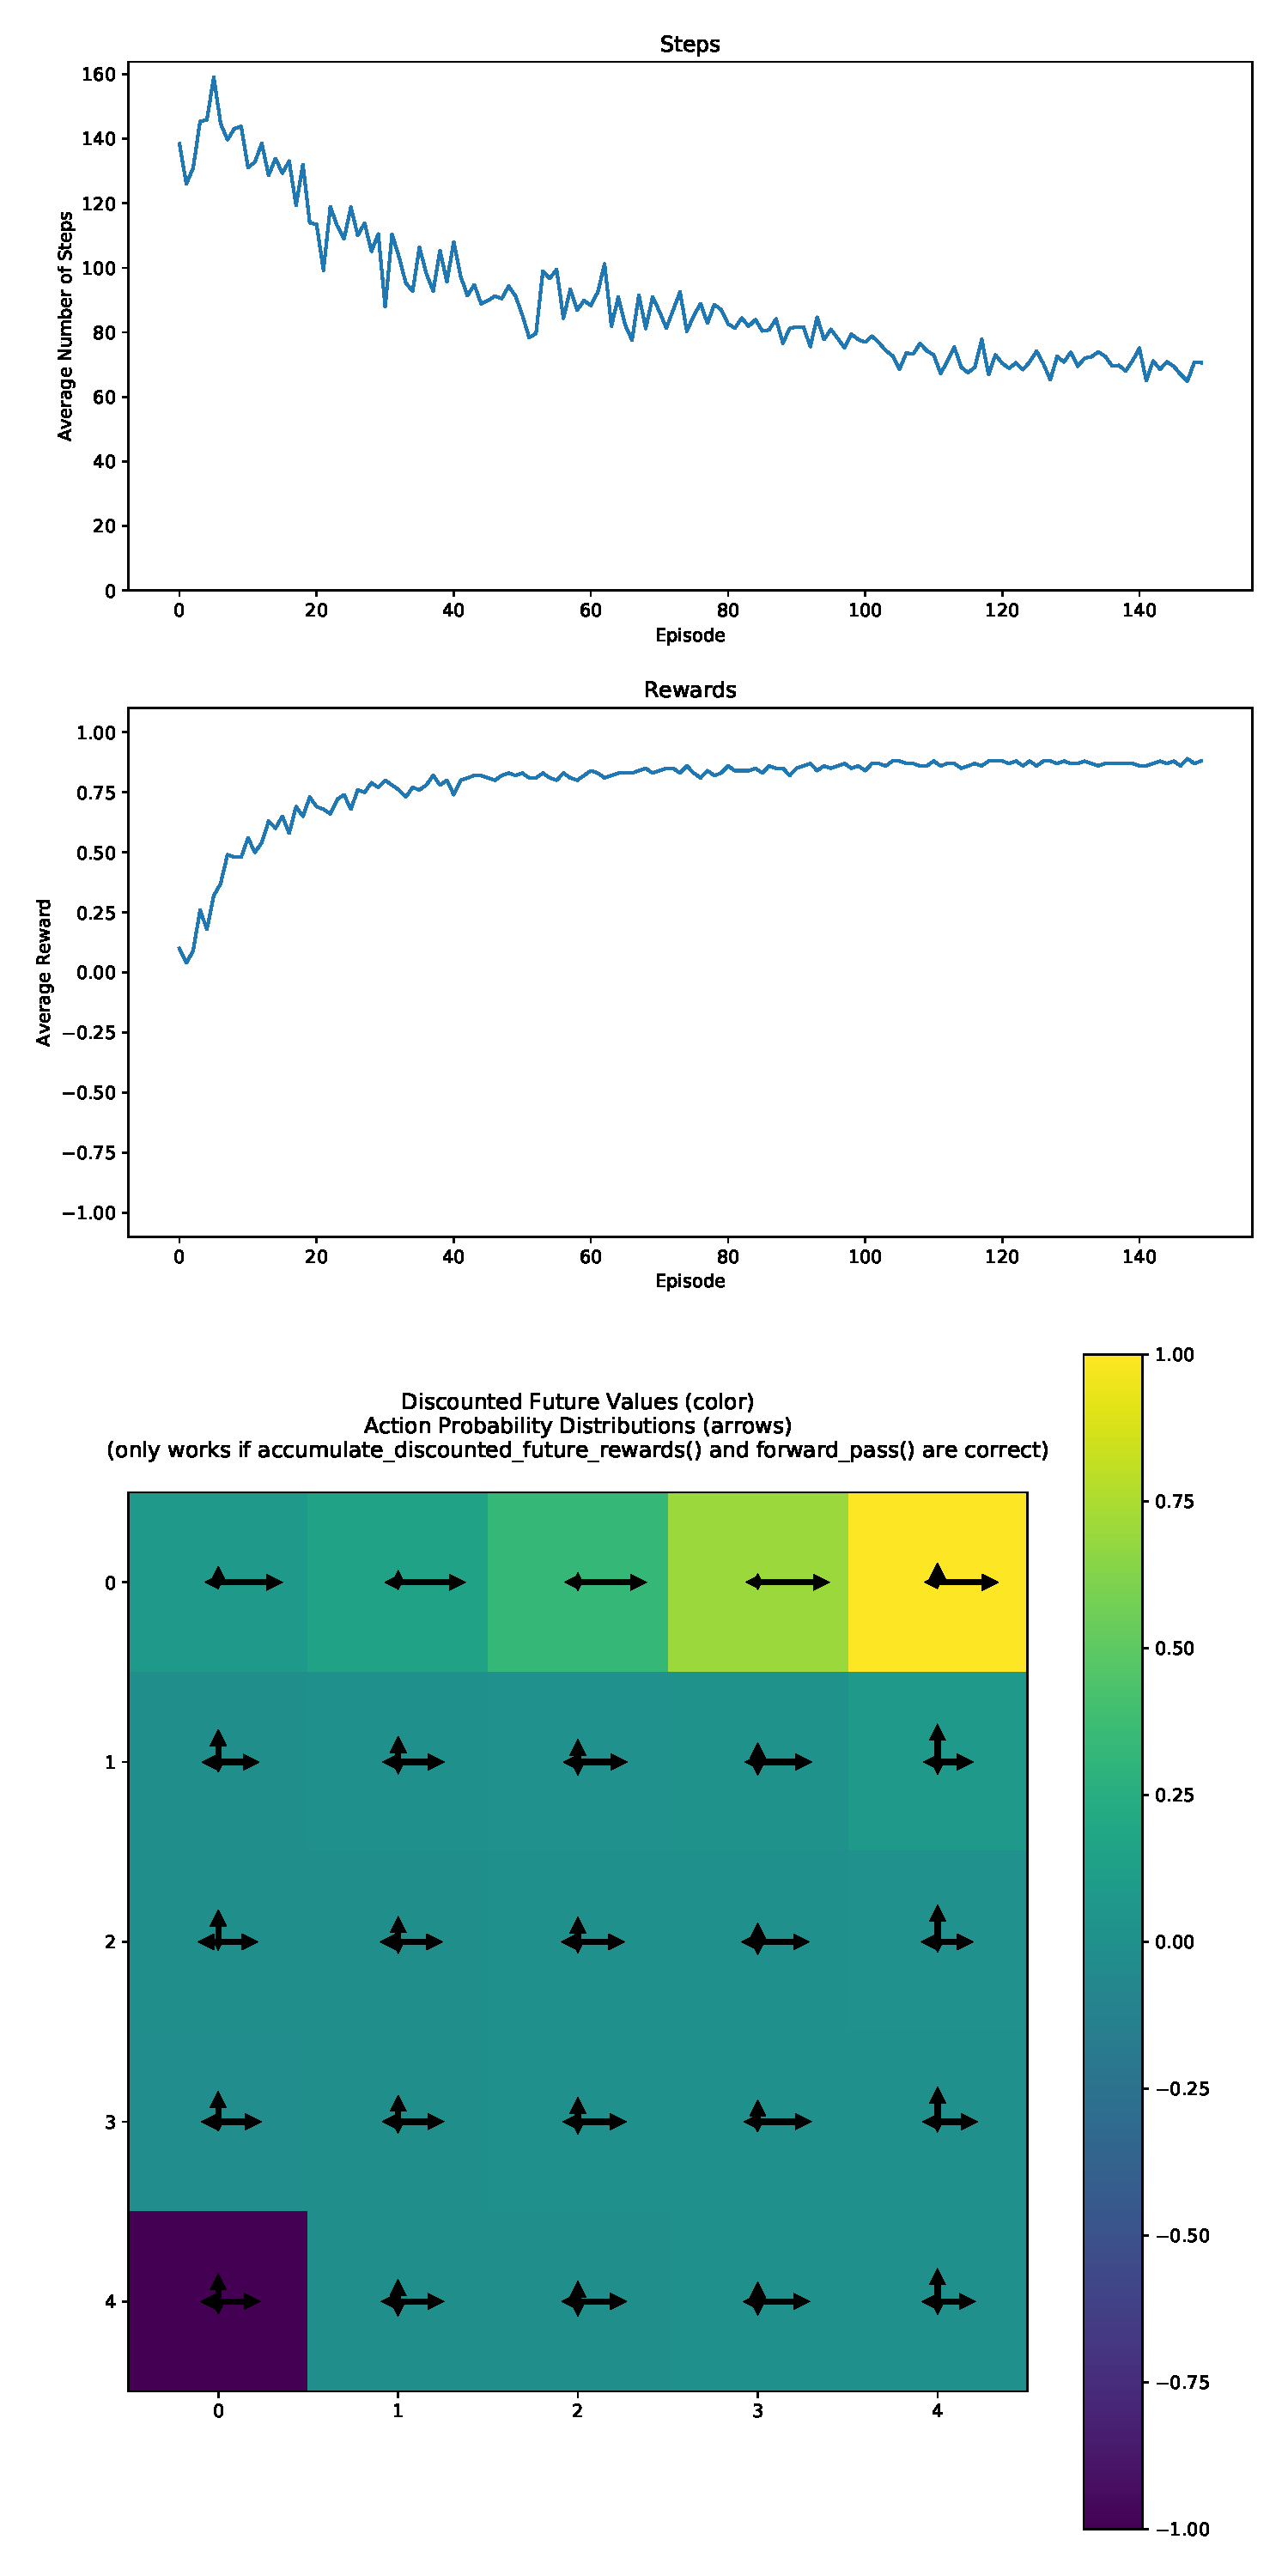
\includegraphics[width=12cm]{policy-gradient/policy_gradient_results.pdf}
\end{center}
